\begin{table}[!htbp]
\begin{adjustwidth}{-0.25in}{0in}
\centering
\caption{\bf MR-specific transcription factor motifs in peaks supported by Mendelian randomization.}
\label{tab:motif}
\begingroup
\scriptsize
\singlespacing
\setlength{\tabcolsep}{1.5pt}
\renewcommand{\arraystretch}{1.15}
\newcolumntype{C}[1]{>{\centering\arraybackslash}m{#1}}
\begin{tabular}{@{}C{1.32in}*{6}{C{0.42in}}>{\raggedright\arraybackslash}m{2.6in}@{}}
\toprule
 & \multicolumn{6}{c}{p.adj} & \\
\cmidrule(lr){2-7}
Motif logo & IVW & MR-Egger & SMR & CCT & WNN & Pseudo\-bulk & Brief interpretation \& link \\
\midrule
\rowcolor{gray!14}\multicolumn{8}{@{}l}{\textbf{Bn}} \\
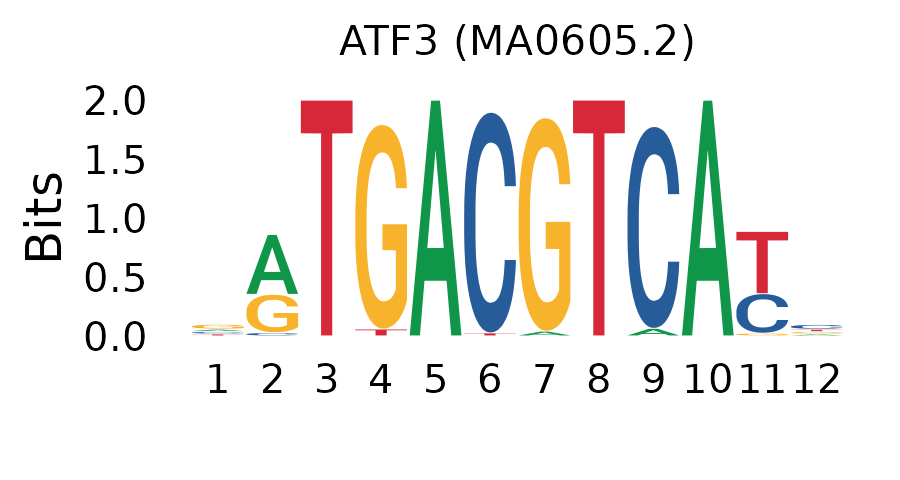
\includegraphics[width=1.3in]{MA0605.2.png} & \textbf{0.041} & \textbf{\mbox{1.5e\(-\)4}} & 0.157 & 0.059 & 0.072 & 0.056 & In mouse marginal zone B cells, ATF3 drives PDL1 expression, through which these cells restrain the T follicular helper response to a high-cholesterol diet. \newline \url{https://pubmed.ncbi.nlm.nih.gov/28414328/} \\
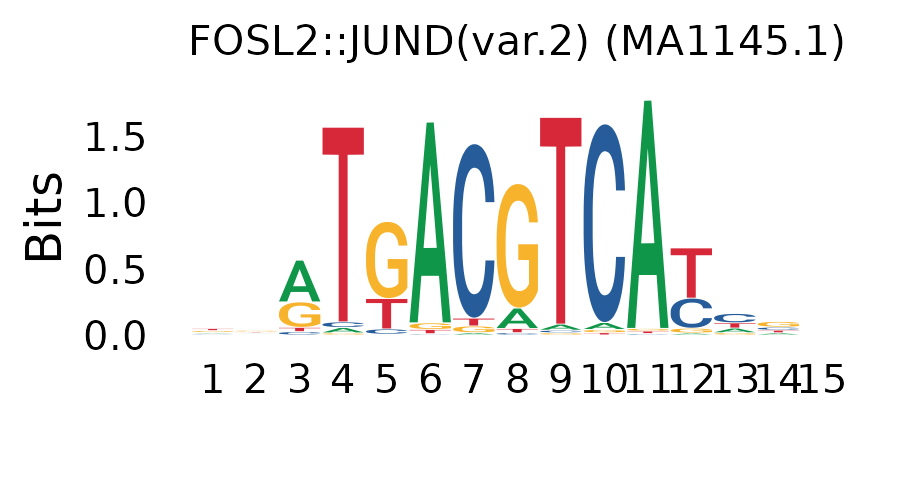
\includegraphics[width=1.3in]{MA1145.1.png} & 0.057 & \textbf{0.001} & 0.137 & 0.056 & 0.088 & 0.059 & Fra-2 (FOSL2) drives IRF4 and Foxo1 transcription and is required for mouse B-cell proliferation and pre-B-cell differentiation. \newline \url{https://pubmed.ncbi.nlm.nih.gov/28566276/} \\
\rowcolor{gray!14}\multicolumn{8}{@{}l}{\textbf{CD4 T cell}} \\
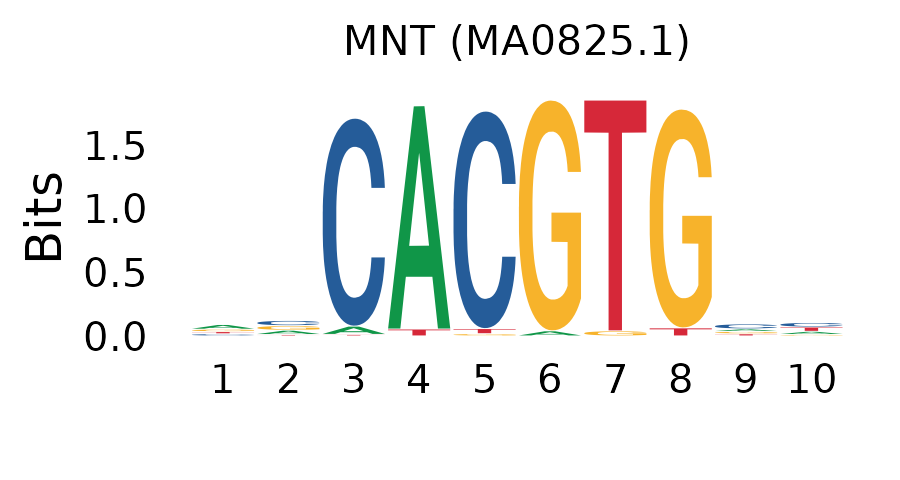
\includegraphics[width=1.3in]{MA0825.1.png} & 0.176 & \textbf{0.003} & 0.051 & \textbf{0.032} & 0.077 & 0.113 & Deleting Mnt in mouse T cells causes Th1-skewed hyperproliferation of activated CD4\(^+\) T cells, intestinal inflammation and T-cell lymphoma. \newline \url{https://pubmed.ncbi.nlm.nih.gov/16507988/} \\
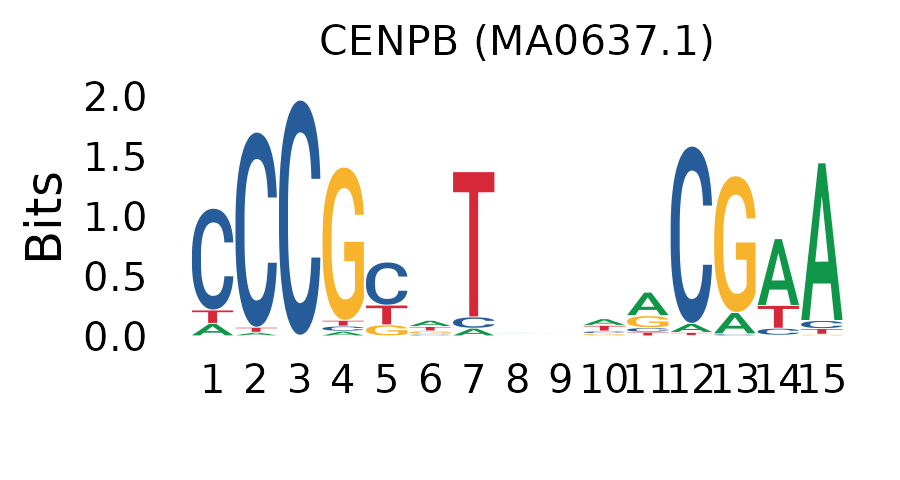
\includegraphics[width=1.3in]{MA0637.1.png} & \textbf{0.035} & \textbf{0.004} & 0.172 & \textbf{0.033} & 0.329 & 0.156 & CENP-B is a major anti-centromere autoantigen; antibodies to recombinant CENP-B were detected in 60\% of patients with primary biliary cholangitis. \newline \url{https://pubmed.ncbi.nlm.nih.gov/8527711/} \\
\rowcolor{gray!14}\multicolumn{8}{@{}l}{\textbf{CD8 T cell}} \\
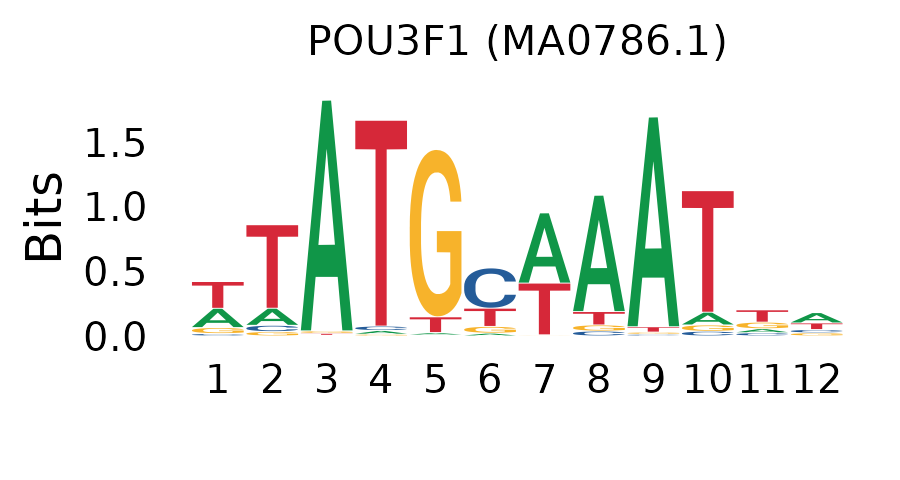
\includegraphics[width=1.3in]{MA0786.1.png} & 0.415 & \textbf{0.006} & 0.591 & 0.140 & 0.499 & 0.232 & POU3F1 is one of the top five transcription factors predicted from disease-associated chromatin accessibility and gene expression in CD4\(^+\) T cells of SLE patients. \newline \url{https://pubmed.ncbi.nlm.nih.gov/36738683/} \\
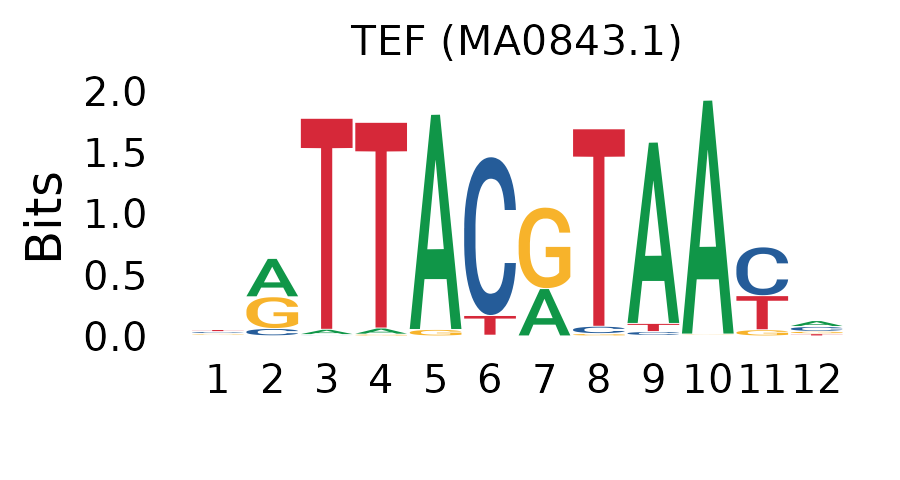
\includegraphics[width=1.3in]{MA0843.1.png} & 0.112 & \textbf{0.010} & 0.067 & 0.124 & 0.117 & 0.087 & TEF is expressed in hematolymphoid progenitors, where it blocks apoptosis on IL-3 withdrawal and restrains proliferation by down-regulating the common beta chain of cytokine receptors. \newline \url{https://pubmed.ncbi.nlm.nih.gov/15665112/} \\
\bottomrule
\end{tabular}
\par\medskip
\begin{minipage}{\linewidth}
\footnotesize
Motif enrichment was tested for peaks selected by each method
(within-gene BH-adjusted \(\q<0.1\)) against a background matched on GC content and accessibility
(Signac, JASPAR2020 vertebrate CORE motifs). MR-specific motifs have p.adj \(<0.05\) and fold
enrichment \(>1\) in at least one of IVW, MR-Egger, and SMR, with no significant enrichment
(p.adj \(\ge0.05\)) in WNN or Pseudobulk; for each cell type, the two with the smallest MR p.adj
and a clear literature-based interpretation are shown. Bold, p.adj \(<0.05\) with fold
enrichment \(>1\). p.adj is the adjusted motif-enrichment p-value reported by Signac for each
method. Each interpretation is based on the single paper linked below it, checked against its
PubMed record.
Pseudobulk, pseudobulk correlation; WNN, WNN metacell correlation;
CCT, Cauchy combination of SMR, IVW, and MR-Egger.
\end{minipage}
\endgroup
\end{adjustwidth}
\end{table}
